\spacing{1.3}


\section{Compuestos químicos}
\begin{minipage}{0.45\textwidth}
    Los electrones de la última capa (electrones de valencia) son los responsables de las propiedades químicas de un elemento, tal como se muestra en la Figura \eqref{fig:atomo_valencia}.
    Los elementos que tienen la misma configuración electrónica en su capa de valencia pertenecen al mismo grupo de la tabla periódica, lo que les confiere propiedades químicas similares.

    Los elementos de la tabla periódica se combinan con otros elementos para conseguir mayor estabilidad, formando compuestos químicos.

\end{minipage}
\hfill
% --- Valence shell diagram (wrapfigure on the right, at section start) ---
\begin{minipage}{0.45\textwidth}
    \begin{figure}[H]
        \vspace{-12pt}
        \centering
        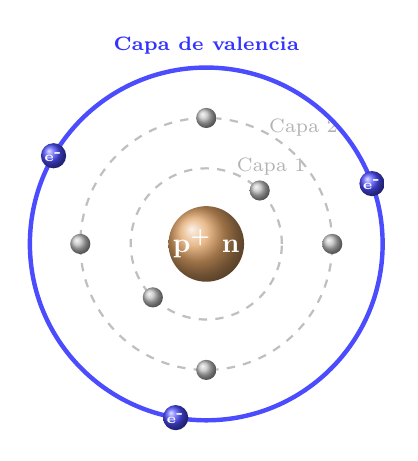
\begin{tikzpicture}[scale=0.40]
            % Nucleus with ochre gradient (only p+ and n)
            \shade[ball color=orange!80!black!60] (0,0) circle (1.2cm);
            \node[font=\normalsize\bfseries, white] at (0,0) {p\textsuperscript{+} n};
            % Shell 1 (radius 2.4)
            \draw[gray!50, thick, dashed] (0,0) circle (2.4cm);
            % Label Shell 1: between shell 1 (2.4) and shell 2 (4.0), at radius ~3.2
            \node[gray!60, font=\scriptsize] at (50:3.2) {Capa 1};
            % Shell 2 (radius 4.0, more separated)
            \draw[gray!50, thick, dashed] (0,0) circle (4.0cm);
            % Label Shell 2: between shell 2 (4.0) and valence (5.6), at radius ~4.8
            \node[gray!60, font=\scriptsize] at (50:4.8) {Capa 2};
            % Valence shell (radius 5.6, highlighted)
            \draw[blue!70, ultra thick] (0,0) circle (5.6cm);
            \node[blue!80, font=\scriptsize\bfseries] at (0, 6.3) {Capa de valencia};
            % Valence electrons (blue)
            \foreach \angle in {20, 150, 260} {
                \shade[ball color=blue!70] (\angle:5.6) circle (0.4cm);
                \node[white, font=\tiny\bfseries] at (\angle:5.6) {e\textsuperscript{-}};
            }
            % Inner electrons shell 1 (gray)
            \foreach \angle in {45, 225} {
                \shade[ball color=gray!50] (\angle:2.4) circle (0.32cm);
            }
            % Inner electrons shell 2 (gray)
            \foreach \angle in {0, 90, 180, 270} {
                \shade[ball color=gray!50] (\angle:4.0) circle (0.32cm);
            }
        \end{tikzpicture}
        \caption{Representación simplificada de un átomo.}
        \label{fig:atomo_valencia}
    \end{figure}
\end{minipage}
%
%    \begin{exercise} Answer the following questions:
%    \begin{enumerate}[label=\letraminuscula]
%        \item What are valence electrons?
%        \item Why do elements in the same group have similar chemical properties?
%        \item Sodium (\ch{Na}) and potassium (\ch{K}) are in the same group of the periodic table. Will they have similar chemical properties? Justify your answer.
%    \end{enumerate}
%    \begin{solu}
%        Answer the following questions:
%        \begin{enumerate}[label=\letraminuscula]
%        \item What are valence electrons?
%        \item Why do elements in the same group have similar chemical properties?
%        \item Sodium (\ch{Na}) and potassium (\ch{K}) are in the same group of the periodic table. Will they have similar chemical properties? Justify your answer.
%        \end{enumerate}
%        \negsubro{SOLUTION:}
%        \begin{enumerate}[label=\letraminuscula]
%            \item Valence electrons are the electrons found in the outermost shell of an atom. They are responsible for the chemical properties of the element.
%            \item Because they have the same electron configuration in their valence shell, that is, the same number of electrons in the outermost shell.
%            \item Yes, sodium and potassium will have similar chemical properties because they belong to the same group (group 1, alkali metals) and therefore have the same number of valence electrons (1 electron).
%        \end{enumerate}
%    \end{solu}
%\end{exercise}
\begin{definition}[Compuesto químico]
    Es una sustancia formada por dos o más elementos diferentes que están unidos químicamente en proporciones fijas.
\end{definition}
También es importante conocer la definición de molécula.
\begin{definition}[Molécula]
    es la unidad más pequeña de una sustancia química que conserva sus propiedades.
\end{definition}
Los diferentes tipos de estructuras que podemos encontrar son:
\begin{enumerate}[label=\numberballmDarkTeal]
        \item \negsubro{Átomos aislados}. \\
        Los átomos aislados se encuentran en los \textbf{gases nobles} debido a su alta estabilidad.
        Los gases nobles no tienden a combinarse con otros elementos porque su capa de valencia ya está completa.

        Los átomos aislados presentan las siguientes \textbf{propiedades físicas y químicas}:
        \begin{itemize}
            \item Son sustancias gaseosas a temperatura ambiente.
            \item No conducen la electricidad.
            \item No reaccionan con otras sustancias.
        \end{itemize}

        \item \negsubro{Moléculas diatómicas homonucleares}. \\
        Son moléculas formadas por dos átomos de un mismo elemento.
        Las moléculas diatómicas homonucleares que se encuentran en la naturaleza son:
        \ch{H2}, \ch{O2}, \ch{N2}, \ch{F2}, \ch{Cl2}, \ch{Br2}, y \ch{I2}.

        \item \negsubro{Moléculas heteronucleares}. \\
        Son moléculas que contienen dos o más elementos diferentes.

        Ejemplos: \ch{HCl}, \ch{H2S}, \ch{H2O}.

        \item \negsubro{Cristales}. \\
        Son sólidos cuyas partículas están dispuestas siguiendo un patrón que se repite en las tres dimensiones del espacio.
        \begin{itemize}
            \item \textbf{Cristales no metálicos}: como el grafito y el diamante, ambos formados por carbono pero con estructuras diferentes.
            \item \textbf{Cristales metálicos}: como el hierro, el cobre, etc.
        \end{itemize}

        % --- Comparative diagram: diamond vs graphite ---
        La Figura \eqref{fig:diamante_grafito} muestra cómo el carbono puede formar dos estructuras cristalinas muy diferentes.

        \begin{figure}[ht]
            \centering
            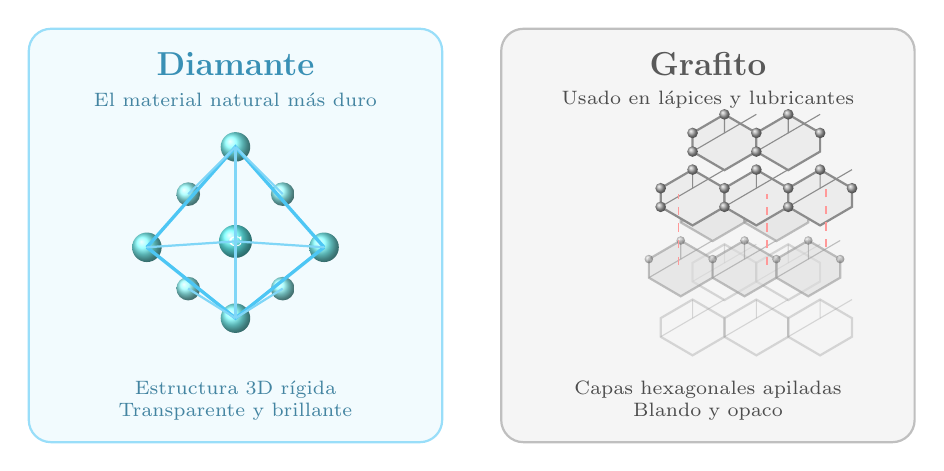
\begin{tikzpicture}[scale=0.75]
                % ===== DIAMOND =====
                % Decorative frame
                \fill[cyan!5, rounded corners=8pt] (-7.5,-1.8) rectangle (-0.5,5.2);
                \draw[cyan!40, thick, rounded corners=8pt] (-7.5,-1.8) rectangle (-0.5,5.2);
                \node[font=\large\bfseries, cyan!70!black] at (-4, 4.6) {Diamante};
                % Hardness icon
                \node[font=\scriptsize, cyan!60!black] at (-4, 4.0) {El material natural más duro};
                % 3D tetrahedral structure with perspective
                % Carbon atoms (shiny spheres)
                \shade[ball color=cyan!50] (-5.5,1.5) circle (0.25);
                \shade[ball color=cyan!50] (-2.5,1.5) circle (0.25);
                \shade[ball color=cyan!50] (-4,3.2) circle (0.25);
                \shade[ball color=cyan!50] (-4,0.3) circle (0.25);
                \shade[ball color=cyan!40] (-4.8,2.4) circle (0.2);

                \shade[ball color=cyan!40] (-3.2,2.4) circle (0.2);
                \shade[ball color=cyan!40] (-4.8,0.8) circle (0.2);
                \shade[ball color=cyan!40] (-3.2,0.8) circle (0.2);
                \shade[ball color=cyan!60] (-4,1.6) circle (0.28);
                \node[white, font=\tiny\bfseries] at (-4,1.6) {C};
                % Strong bonds (thick lines)
                \draw[cyan!70, very thick] (-5.5,1.5)--(-4,3.2)--(-2.5,1.5);
                \draw[cyan!70, very thick] (-5.5,1.5)--(-4,0.3)--(-2.5,1.5);
                \draw[cyan!70, very thick] (-4,3.2)--(-4,0.3);
                \draw[cyan!50, thick] (-4,1.6)--(-5.5,1.5);
                \draw[cyan!50, thick] (-4,1.6)--(-2.5,1.5);
                \draw[cyan!50, thick] (-4,1.6)--(-4,3.2);
                \draw[cyan!50, thick] (-4,1.6)--(-4,0.3);
                \draw[cyan!50, thick] (-4.8,2.4)--(-4,3.2);
                \draw[cyan!50, thick] (-3.2,2.4)--(-4,3.2);
                \draw[cyan!50, thick] (-4.8,0.8)--(-4,0.3);
                \draw[cyan!50, thick] (-3.2,0.8)--(-4,0.3);
                % Properties
                \node[font=\scriptsize, text width=3cm, align=center, cyan!60!black] at (-4,-1.1) {Estructura 3D rígida \\ Transparente y brillante};

                % ===== GRAPHITE =====
                \fill[gray!8, rounded corners=8pt] (0.5,-1.8) rectangle (7.5,5.2);
                \draw[gray!50, thick, rounded corners=8pt] (0.5,-1.8) rectangle (7.5,5.2);
                \node[font=\large\bfseries, gray!70!black] at (4, 4.6) {Grafito};
                \node[font=\scriptsize, gray!60!black] at (4, 4.0) {Usado en lápices y lubricantes};
                % Lower layer (lighter, depth effect)
                \begin{scope}[shift={(3.2,0.3)}, scale=0.9, opacity=0.35]
                    \foreach \hx/\hy in {0/0, 1.2/0, 2.4/0, 0.6/1.04, 1.8/1.04} {
                        \draw[gray!80, thick]
                        (\hx,\hy) -- ++(0.6,0.35) -- ++(0.6,-0.35)
                        -- ++(0,-0.35) -- ++(-0.6,-0.35) -- ++(-0.6,0.35) -- cycle;
                        \draw[gray!80] (\hx+0.6,\hy+0.35) -- ++(0,-0.35) -- ++(-0.6,-0.35);
                        \draw[gray!80] (\hx+0.6,\hy) -- ++(0.6,0.35);
                    }
                \end{scope}
                % Middle layer
                \begin{scope}[shift={(3.0,1.3)}, scale=0.9, opacity=0.6]
                    \foreach \hx/\hy in {0/0, 1.2/0, 2.4/0, 0.6/1.04, 1.8/1.04} {
                        \fill[gray!25]
                        (\hx,\hy) -- ++(0.6,0.35) -- ++(0.6,-0.35)
                        -- ++(0,-0.35) -- ++(-0.6,-0.35) -- ++(-0.6,0.35) -- cycle;
                        \draw[gray!80, thick]
                        (\hx,\hy) -- ++(0.6,0.35) -- ++(0.6,-0.35)
                        -- ++(0,-0.35) -- ++(-0.6,-0.35) -- ++(-0.6,0.35) -- cycle;
                        \draw[gray!80] (\hx+0.6,\hy+0.35) -- ++(0,-0.35) -- ++(-0.6,-0.35);
                        \draw[gray!80] (\hx+0.6,\hy) -- ++(0.6,0.35);
                    }
                    % Atoms at vertices of middle layer
                    \foreach \ax/\ay in {0/0, 0.6/0.35, 1.2/0, 1.8/0.35, 2.4/0, 3.0/0.35, 3.6/0,
                    0.6/1.04, 1.2/1.39, 1.8/1.04, 2.4/1.39, 3.0/1.04} {
                        \shade[ball color=gray!55] (\ax,\ay) circle (0.08);
                    }
                \end{scope}
                % Top layer (darker, foreground)
                \begin{scope}[shift={(3.2,2.5)}, scale=0.9]
                    \foreach \hx/\hy in {0/0, 1.2/0, 2.4/0, 0.6/1.04, 1.8/1.04} {
                        \fill[gray!15]
                        (\hx,\hy) -- ++(0.6,0.35) -- ++(0.6,-0.35)
                        -- ++(0,-0.35) -- ++(-0.6,-0.35) -- ++(-0.6,0.35) -- cycle;
                        \draw[gray!90, thick]
                        (\hx,\hy) -- ++(0.6,0.35) -- ++(0.6,-0.35)
                        -- ++(0,-0.35) -- ++(-0.6,-0.35) -- ++(-0.6,0.35) -- cycle;
                        \draw[gray!90] (\hx+0.6,\hy+0.35) -- ++(0,-0.35) -- ++(-0.6,-0.35);
                        \draw[gray!90] (\hx+0.6,\hy) -- ++(0.6,0.35);
                    }
                    % Atoms at vertices of top layer
                    \foreach \ax/\ay in {0/0, 0.6/0.35, 1.2/0, 1.8/0.35, 2.4/0, 3.0/0.35, 3.6/0,
                    0/-0.35, 1.2/-0.35, 2.4/-0.35,
                    0.6/1.04, 1.2/1.39, 1.8/1.04, 2.4/1.39, 3.0/1.04,
                    0.6/0.69, 1.8/0.69} {
                        \shade[ball color=gray!70] (\ax,\ay) circle (0.1);
                    }
                \end{scope}
                % Separation lines between layers (weak forces)
                \draw[red!40, dashed, thin] (3.5,1.2) -- (3.5,2.4);
                \draw[red!40, dashed, thin] (5.0,1.2) -- (5.0,2.4);
                \draw[red!40, dashed, thin] (6.0,1.5) -- (6.0,2.6);
                % Properties
                \node[font=\scriptsize, text width=4cm, align=center, gray!60!black] at (4,-1.1) {Capas hexagonales apiladas \\ Blando y opaco};
            \end{tikzpicture}
            \caption{El diamante y el grafito están hechos de carbono, pero sus diferentes estructuras les confieren propiedades muy distintas.}
            \label{fig:diamante_grafito}
        \end{figure}
\end{enumerate}


\section{Enlace químico}

Los átomos de diferentes elementos se unen para formar moléculas. Esta unión se llama \azul{\texttt{enlace químico}}. El enlace químico se produce porque la molécula formada es más estable que los átomos aislados.

En la naturaleza podemos encontrar principalmente 3 tipos de enlaces:

\begin{enumerate}[label=\numberballmDarkTeal]
\item \negsubro{Enlace iónico}: se produce por transferencia de electrones. Un elemento pierde electrones y otro los gana, formando un catión (ion positivo) y un anión (ion negativo). Ambos iones se mantienen unidos por la fuerza eléctrica de atracción.

Por ejemplo, el \ch{NaCl} se forma porque el \ch{Na} pierde un \el{} y se convierte en \ch{Na+}, mientras que el \ch{Cl} gana ese \el{} y se convierte en \ch{Cl-}, dando lugar a \ch{Na+ Cl-} (Figura \eqref{fig:enlace_ionico}).

% --- Ionic bond diagram ---
\begin{figure}[ht]
    \centering
    \begin{tikzpicture}[scale=0.85]
% Title
        \node[font=\bfseries\large, orange!70!black] at (1.5,3.9) {Formación del enlace iónico: \ch{NaCl}};

% === BEFORE ===
        \node[font=\small\bfseries, gray] at (-5.5,2.3) {ANTES};

% Na with electron shells
        \shade[ball color=blue!40] (-4.5,0) circle (0.6);
        \node[white, font=\bfseries] at (-4.5,0) {Na};
% Na valence shell (1 electron)
        \draw[blue!50, thick] (-4.5,0) circle (1.3);
        \shade[ball color=red!70] (-4.5,1.3) circle (0.15);
        \node[font=\tiny, blue!70] at (-4.5,-1.7) {11 e\textsuperscript{-} (2, 8, \textbf{1})};

% Cl with electron shells
        \shade[ball color=green!60!black!40] (-1.5,0) circle (0.7);
        \node[white, font=\bfseries] at (-1.5,0) {Cl};
% Cl valence shell (7 electrons)
        \draw[green!60!black, thick] (-1.5,0) circle (1.4);
        \foreach \a in {0,51.4,102.8,154.3,205.7,257.1,308.6} {
            \shade[ball color=red!70] ({-1.5+1.4*cos(\a)},{1.4*sin(\a)}) circle (0.15);
        }
        \node[font=\tiny, green!50!black] at (-1.5,-1.7) {17 e\textsuperscript{-} (2, 8, \textbf{7})};

% Transfer arrow (curved, with correct tip)
        \draw[-{Stealth[length=8pt, width=5pt]}, ultra thick, red!70, decorate, decoration={snake, amplitude=1.5pt, segment length=8pt, post length=8pt}]
        (-4.5,1.6) .. controls (-3,2.8) and (-2,2.8) .. (-1.5,1.7);
        \node[font=\small\bfseries, red!70] at (-3,3.0) {1 e\textsuperscript{-}};

% === Central arrow ===
        \draw[->, ultra thick, orange!70, >=stealth] (0.8,0) -- (2.2,0);
        \node[font=\tiny\bfseries, orange!70] at (1.5,0.4) {Forma};

% === AFTER ===
        \node[font=\small\bfseries, gray] at (5.5,2.3) {DESPUÉS};

% Na+ (smaller, lost electron)
        \shade[ball color=blue!60] (4,0) circle (0.5);
        \node[white, font=\bfseries] at (4,0) {Na\textsuperscript{+}};
% Decorative + sign
        \node[blue!70, font=\Large\bfseries] at (4,1.0) {$+$};

% Cl- (larger, gained electron)
        \shade[ball color=green!60!black!40] (7,0) circle (0.8);
        \node[white, font=\bfseries] at (7,0) {Cl\textsuperscript{-}};
% Decorative - sign
        \node[green!50!black, font=\Large\bfseries] at (7,1.2) {$-$};

% Attraction force (rays)
        \foreach \dy in {-0.3,0,0.3} {
            \draw[orange!80, thick, <->, >=stealth] (4.6,\dy) -- (6.1,\dy);
        }
        \node[font=\tiny\bfseries, orange!80] at (5.35,-0.8) {Atracción eléctrica};

% Final configuration
        \node[font=\tiny, blue!70] at (4,-1.7) {10 e\textsuperscript{-} (2, 8)};
        \node[font=\tiny, green!50!black] at (7,-1.7) {18 e\textsuperscript{-} (2, 8, 8)};

% Stability note
        \node[font=\tiny, gray, text width=3cm, align=center] at (5.5,-2.8) {Ambos tienen ahora \\ 8 e\textsuperscript{-} en su última capa};
    \end{tikzpicture}
    \caption{Formación del enlace iónico en el \ch{NaCl}. El sodio transfiere un electrón al cloro, formando iones que se atraen entre sí.}
    \label{fig:enlace_ionico}
\end{figure}

\item \negsubro{Enlace covalente}: es el enlace que se forma cuando dos átomos comparten electrones. El enlace formado se representa con una línea (\ch{-}), aunque a veces se omite por simplicidad.

Por ejemplo, el \ch{H} y el \ch{Cl} comparten electrones para formar un enlace covalente: \ch{H-Cl} (Figura \eqref{fig:enlace_covalente}).

% --- Covalent bond diagram ---
\begin{figure}[ht]
    \centering
    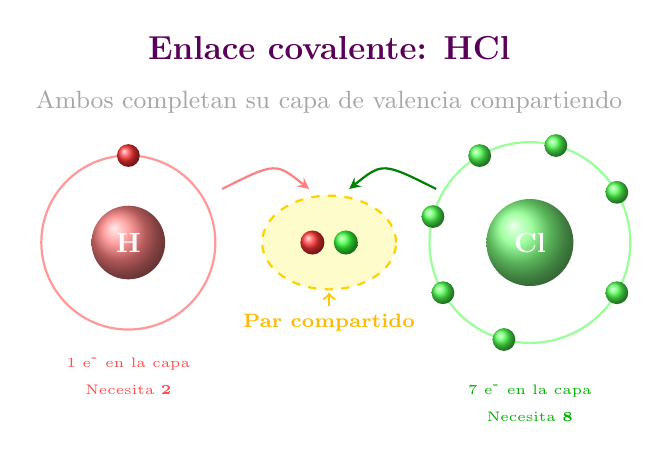
\begin{tikzpicture}[scale=0.85]
% Background
%\fill[violet!3, rounded corners=10pt] (-6,-3.5) rectangle (6,3.5);
% Title
        \node[font=\bfseries\large, violet!70!black] at (0,2.9) {Enlace covalente: \ch{HCl}};

% === H (left) ===
% H electron shell
        \draw[red!40, thick] (-3,0) circle (1.3);
        \shade[ball color=red!50] (-3,0) circle (0.55);
        \node[white, font=\bfseries] at (-3,0) {H};
% H's own electron
        \shade[ball color=red!80] (-3,1.3) circle (0.17);
        \node[font=\tiny, red!70] at (-3,-1.8) {1 e\textsuperscript{-} en la capa};
        \node[font=\tiny, red!70] at (-3,-2.2) {Necesita \textbf{2}};

% === Cl (right) ===
        \draw[green!40, thick] (3,0) circle (1.5);
        \shade[ball color=green!50] (3,0) circle (0.65);
        \node[white, font=\bfseries] at (3,0) {Cl};
% Cl's 7 valence electrons
        \foreach \a/\c in {30/green!70, 75/green!70, 120/green!70, 165/green!70, 210/green!70, 255/green!70, 330/green!70} {
            \shade[ball color=\c] ({3+1.5*cos(\a)},{1.5*sin(\a)}) circle (0.17);
        }
        \node[font=\tiny, green!70!black] at (3,-2.2) {7 e\textsuperscript{-} en la capa};
        \node[font=\tiny, green!70!black] at (3,-2.6) {Necesita \textbf{8}};

% === Sharing zone (center) ===
        \fill[yellow!40, opacity=0.5] (0,0) ellipse (1.0 and 0.7);
        \draw[yellow!70!orange, thick, dashed] (0,0) ellipse (1.0 and 0.7);
% Shared electron pair
        \shade[ball color=red!80] (-0.25,0) circle (0.18);
        \shade[ball color=green!80] (0.25,0) circle (0.18);
% Label
        \node[font=\scriptsize\bfseries, yellow!50!orange, fill=white, inner sep=2pt, rounded corners] at (0,-1.2) {Par compartido};
        \draw[->, yellow!60!orange, thick] (0,-0.95) -- (0,-0.75);

% Approach arrows
        \draw[->, thick, red!50, >=stealth] (-1.6,0.8) .. controls (-0.8,1.2) .. (-0.3,0.8);
        \draw[->, thick, green!50!black, >=stealth] (1.6,0.8) .. controls (0.8,1.2) .. (0.3,0.8);

% Result below
        \node[font=\small, gray!70, fill=white, inner sep=3pt, rounded corners=3pt] at (0,2.1)
            {Ambos completan su capa de valencia compartiendo};
    \end{tikzpicture}
    \caption{Enlace covalente en el \ch{HCl}. Ambos átomos comparten un par de electrones para completar su capa de valencia.}
    \label{fig:enlace_covalente}
\end{figure}

\item \negsubro{Enlace metálico}: es el enlace que se forma entre átomos de elementos metálicos. Los átomos de un metal comparten sus electrones de valencia, que se mueven libremente entre todos los átomos formando una ``nube de electrones''. Esto explica por qué los metales conducen la electricidad.

% --- Metallic bond diagram ---
La Figura \eqref{fig:enlace_metalico} ilustra este tipo de enlace.

\begin{figure}[ht]
    \centering
    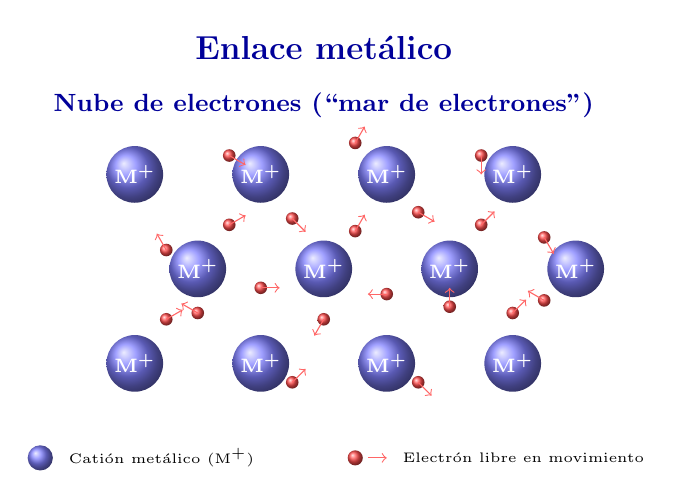
\begin{tikzpicture}[scale=0.8]
% General background
%\fill[blue!3, rounded corners=10pt] (-3.5,-3.5) rectangle (7.5,4.5);
% Title
        \node[font=\bfseries\large, blue!60!black] at (2,3.5) {Enlace metálico};

% Electron cloud (vibrant yellow background)
%\fill[yellow!25, rounded corners=12pt] (-2.5,-2.5) rectangle (6.5,3.0);
%\fill[yellow!15, rounded corners=12pt] (-2.8,-2.8) rectangle (6.8,3.2);
%\draw[yellow!60, thick, dashed, rounded corners=12pt] (-2.8,-2.8) rectangle (6.8,3.2);
        \node[font=\small\bfseries, blue!60!black, inner sep=3pt, rounded corners=3pt] at (2,2.6) {Nube de electrones (``mar de electrones'')};

% Lattice of metallic cations (ordered arrangement)
        \foreach \x/\y in {-1/-1.5, 1/-1.5, 3/-1.5, 5/-1.5, 0/0, 2/0, 4/0, 6/0, -1/1.5, 1/1.5, 3/1.5, 5/1.5} {
            \shade[ball color=blue!50] (\x,\y) circle (0.45);
            \node[white, font=\scriptsize\bfseries] at (\x,\y) {M\textsuperscript{+}};
        }

% Free electrons moving (with arrows to indicate movement)
        \foreach \x/\y/\ang in {
            0.5/0.7/30, 1.5/0.8/-45, 2.5/0.6/60, 3.5/0.9/-30,
            4.5/0.7/45, -0.5/0.3/120, 5.5/0.5/-60,
            0/-0.7/150, 2/-0.8/-120, 4/-0.6/90,
            1/-0.3/0, 3/-0.4/180, 5/-0.7/45,
            0.5/1.8/-30, 2.5/2.0/60, 4.5/1.8/-90,
            -0.5/-0.8/30, 5.5/-0.5/150, 1.5/-1.8/45, 3.5/-1.8/-45
        } {
            \shade[ball color=red!70] (\x,\y) circle (0.1);
            \draw[->, red!60, thin] (\x,\y) -- ++(\ang:0.3);
        }

% Legend
        \shade[ball color=blue!50] (-2.5,-3.0) circle (0.2);
        \node[font=\tiny, right] at (-2.2,-3.0) {Catión metálico (M\textsuperscript{+})};
        \shade[ball color=red!70] (2.5,-3.0) circle (0.12);
        \draw[->, red!60, thin] (2.7,-3.0) -- ++(0:0.3);
        \node[font=\tiny, right] at (3.1,-3.0) {Electrón libre en movimiento};
    \end{tikzpicture}
    \caption{En el enlace metálico, los cationes metálicos están rodeados por una nube de electrones en movimiento libre, lo que explica la conductividad eléctrica.}
    \label{fig:enlace_metalico}
\end{figure}

\end{enumerate}


\section{Masa atómica y masa molecular}

\subsection{Masa atómica}
Los átomos son partículas muy pequeñas, por lo que si midiéramos su masa en kilogramos, obtendríamos valores extremadamente pequeños. Por eso se creó una unidad especial que nos permite trabajar con estas masas de forma más sencilla.

Esta unidad se llama \azul{\texttt{unidad de masa atómica (uma)}} y se representa con \unit{\uma}.

\begin{definition}[Unidad de masa atómica]
    Es una doceava parte (\( \frac{1}{12} \)) de la masa de un átomo de \isotope{C}. Podemos decir que \( \qty{1}{\uma} \approx \qty{1.67e-27}{\kilogram} \).
\end{definition}

En muchos casos, la unidad de masa atómica se omite y solo se indica el número.

En la tabla periódica podemos encontrar las masas atómicas de cada elemento en uma.

Si quisiéramos saber la masa de un átomo en kilogramos, tendríamos que convertir uma a kilogramos utilizando la equivalencia dada anteriormente.

\subsection{Masa molecular}

Si lo que tenemos es una molécula, debemos calcular su masa molecular, es decir, la suma de las masas atómicas de todos los átomos que forman esa molécula. La masa molecular también se expresa en uma.

\begin{example}{}
    Vamos a calcular la masa molecular del \ch{H2O} sabiendo que las masas atómicas de los elementos son \( \ch{H} = 1 \) y \( \ch{O} = 16 \).
    \[
        \ch{H2O} \left\{\rule{0pt}{0.8cm}
                     \begin{array}{lcl}
                         \ch{H} &=& 2 \times \qty{1}{\uma} = \qty{2}{\uma} \\
                         \ch{O} &=& 1 \times \qty{16}{\uma} = \qty{16}{\uma} \\
                         \cline{1-3}
                         \multicolumn{3}{r}{\textbf{Total} = \qty{18}{\uma}}
                     \end{array}
        \right.
    \]
\end{example}

\begin{example}{}
    Vamos a calcular la masa molecular del \ch{H2SO4} sabiendo que las masas atómicas de los elementos son \( \ch{H} = 1 \), \( \ch{O} = 16 \), y \( \ch{S} = 32 \).
    \[
        \ch{H2SO4} \left\{\rule{0pt}{0.8cm}
                       \begin{array}{lcl}
                           \ch{H} &=& 2 \times \qty{1}{\uma} = \qty{2}{\uma} \\
                           \ch{S} &=& 1 \times \qty{32}{\uma} = \qty{32}{\uma} \\
                           \ch{O} &=& 4 \times \qty{16}{\uma} = \qty{64}{\uma} \\
                           \cline{1-3}
                           \multicolumn{3}{r}{\textbf{Total} = \qty{98}{\uma}}
                       \end{array}
        \right.
    \]
\end{example}



\begin{exercise}
    Indica cuál es la forma correcta de calcular la masa molecular del sulfato de calcio, \ch{CaSO4}:
    \begin{enumerate}[label=\letraminuscula]
\item Masa atómica del calcio + masa atómica del azufre + masa atómica del oxígeno.
\item Masa atómica del calcio + masa atómica del azufre + cuatro veces la masa atómica del oxígeno.
    \end{enumerate}
    \begin{solu}
        Indica cuál es la forma correcta de calcular la masa molecular del sulfato de calcio, \ch{CaSO4}:
        \begin{enumerate}[label=\letraminuscula]
\item Masa atómica del calcio + masa atómica del azufre + masa atómica del oxígeno.
\item Masa atómica del calcio + masa atómica del azufre + cuatro veces la masa atómica del oxígeno.
        \end{enumerate}
        Indica cuál es la forma correcta de calcular la masa molecular del sulfato de calcio, \ch{CaSO4}:

        La respuesta correcta es la \textbf{b)}: masa atómica del calcio + masa atómica del azufre + cuatro veces la masa atómica del oxígeno.

        En la fórmula \ch{CaSO4}, el subíndice 4 indica que hay 4 átomos de oxígeno, por lo que debemos multiplicar la masa atómica del oxígeno por 4.
    \end{solu}
\end{exercise}

\begin{exercise}
    El aire, compuesto principalmente por nitrógeno (\ch{N2}) y oxígeno (\ch{O2}), contiene cantidades variables de dióxido de carbono (\ch{CO2}). Busca las masas atómicas en la tabla periódica y calcula la masa molecular de estos tres gases.
    \begin{solu}
        El aire, compuesto principalmente por nitrógeno (\ch{N2}) y oxígeno (\ch{O2}), contiene cantidades variables de dióxido de carbono (\ch{CO2}). Busca las masas atómicas en la tabla periódica y calcula la masa molecular de estos tres gases.
        Calcula la masa molecular del \ch{N2}, \ch{O2}, y \ch{CO2}.

        Masas atómicas: \( \ch{N} = 14 \); \( \ch{O} = 16 \); \( \ch{C} = 12 \).

        \begin{itemize}
            \item \ch{N2}: \( 2 \times 14 = \qty{28}{\uma} \)
            \item \ch{O2}: \( 2 \times 16 = \qty{32}{\uma} \)
            \item \ch{CO2}: \( 1 \times 12 + 2 \times 16 = 12 + 32 = \qty{44}{\uma} \)
        \end{itemize}
    \end{solu}
\end{exercise}

\begin{exercise}
    Calcula la masa molecular del óxido de cinc (\ch{ZnO}), el nitrato de potasio (\ch{KNO3}), el sulfato de calcio (\ch{CaSO4}), el butano (\ch{C4H10}), y el carbonato de calcio (\ch{CaCO3}).
    \begin{solu}
        Calcula la masa molecular del óxido de cinc (\ch{ZnO}), el nitrato de potasio (\ch{KNO3}), el sulfato de calcio (\ch{CaSO4}), el butano (\ch{C4H10}), y el carbonato de calcio (\ch{CaCO3}).

        Calcula la masa molecular del \ch{ZnO}, \ch{KNO3}, \ch{CaSO4}, \ch{C4H10}, y \ch{CaCO3}.

        Masas atómicas: \( \ch{Zn} = 65 \); \( \ch{O} = 16 \); \( \ch{K} = 39 \); \( \ch{N} = 14 \); \( \ch{Ca} = 40 \); \( \ch{S} = 32 \); \( \ch{C} = 12 \); \( \ch{H} = 1 \).
        \begin{itemize}
            \item \ch{ZnO}: \( 65 + 16 = \qty{81}{\uma} \)
            \item \ch{KNO3}: \( 39 + 14 + 3 \times 16 = 39 + 14 + 48 = \qty{101}{\uma} \)
            \item \ch{CaSO4}: \( 40 + 32 + 4 \times 16 = 40 + 32 + 64 = \qty{136}{\uma} \)
            \item \ch{C4H10}: \( 4 \times 12 + 10 \times 1 = 48 + 10 = \qty{58}{\uma} \)
            \item \ch{CaCO3}: \( 40 + 12 + 3 \times 16 = 40 + 12 + 48 = \qty{100}{\uma} \)
        \end{itemize}
    \end{solu}
\end{exercise}

\begin{exercise}
    Busca las masas atómicas en la tabla periódica de esta unidad y ordena los siguientes compuestos de mayor a menor porcentaje de oxígeno: \ch{BaO}, \ch{K2O}, y \ch{CO2}.
    \begin{solu}
        Busca las masas atómicas en la tabla periódica de esta unidad y ordena los siguientes compuestos de mayor a menor porcentaje de oxígeno: \ch{BaO}, \ch{K2O}, y \ch{CO2}.

        Ordena \ch{BaO}, \ch{K2O}, y \ch{CO2} de mayor a menor porcentaje de oxígeno.

        Masas atómicas: \( \ch{Ba} = 137 \); \( \ch{K} = 39 \); \( \ch{C} = 12 \); \( \ch{O} = 16 \).

        \begin{itemize}
            \item \ch{BaO}: masa molecular \( = 137 + 16 = \qty{153}{\uma} \). Porcentaje de O \( = \frac{16}{153} \times 100 = 10.5 \% \)
            \item \ch{K2O}: masa molecular \( = 2 \times 39 + 16 = \qty{94}{\uma} \). Porcentaje de O \( = \frac{16}{94} \times 100 = 17{,}0\% \)
            \item \ch{CO2}: masa molecular \( = 12 + 2 \times 16 = \qty{44}{\uma} \). Porcentaje de O \( = \frac{32}{44} \times 100 = 72{,}7\% \)
        \end{itemize}

        Orden de mayor a menor porcentaje de oxígeno: \ch{CO2} > \ch{K2O} > \ch{BaO}.
    \end{solu}
\end{exercise}


\begin{exercise}
    Indica cuál de estas dos sustancias tiene mayor porcentaje de potasio: el cloruro de potasio (\ch{KCl}) o el nitrato de potasio (\ch{KNO3}).
    \begin{solu}
        Indica cuál de estas dos sustancias tiene mayor porcentaje de potasio: el cloruro de potasio (\ch{KCl}) o el nitrato de potasio (\ch{KNO3}).

        ¿Cuál tiene mayor porcentaje de potasio, el \ch{KCl} o el \ch{KNO3}?

        Masas atómicas: \( \ch{K} = 39 \); \( \ch{Cl} = 35{,}5 \); \( \ch{N} = 14 \); \( \ch{O} = 16 \).

        \begin{itemize}
            \item \ch{KCl}: masa molecular \( = 39 + \num{35.5} = \qty{74.5}{\uma} \). Porcentaje de K \( = \frac{39}{74.5} \times 100 = 52.3\% \)
            \item \ch{KNO3}: masa molecular \( = 39 + 14 + 3 \times 16 = \qty{101}{\uma} \). Porcentaje de K \( = \frac{39}{101} \times 100 = 38.6\% \)
        \end{itemize}

        El \ch{KCl} tiene mayor porcentaje de potasio (52.3\,\%) que el \ch{KNO3} (38.6\,\%).
    \end{solu}
\end{exercise}


\section{Cantidad de sustancia: el mol}

Dado que los átomos son muy pequeños y la materia está formada por cantidades enormes de ellos, se creó una unidad para agrupar muchos átomos y así poder trabajar con cantidades más fáciles de manejar.

Con este propósito se creó la unidad de sustancia llamada \azul{\texttt{mol}} y se representa con \( \bm{n} \).

\begin{definition}[Mol]
    Es la cantidad de sustancia que contiene \num{6.022e23} entidades elementales, que pueden ser átomos, moléculas, iones, electrones, u otras partículas.
\end{definition}

Podemos entender el mol como una ``caja'' que siempre contiene \num{6.022e23} ``cosas''.

Este número tan grande se llama \azul{\texttt{constante de Avogadro}} y se representa con \( \bm{N_A} \).

\begin{equation*}
    N_A = \num{6.022e23}\ \dfrac{\text{partículas}}{\unit{\mol}}
\end{equation*}

% --- Visual diagram of the mole ---
La Figura \eqref{fig:mol_particulas} ilustra este concepto.

\begin{figure}[ht]
    \centering
    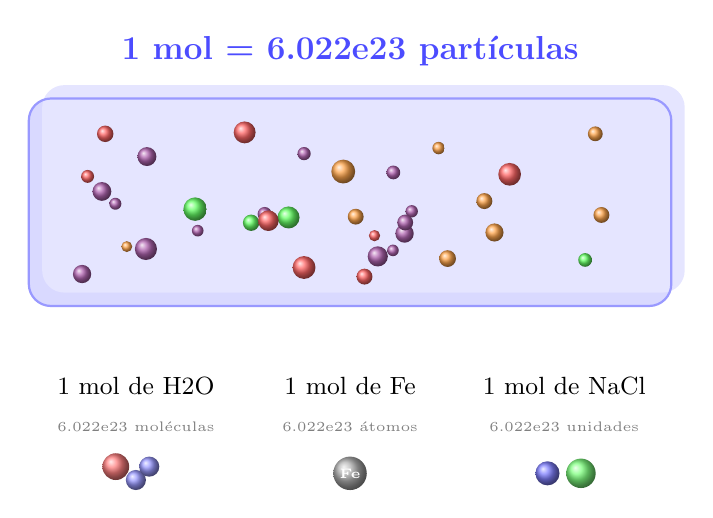
\begin{tikzpicture}[scale=0.85]
% General background
%\fill[blue!3, rounded corners=12pt] (-5.5,-3.5) rectangle (5.5,4.5);

% Large title
        \node[font=\large\bfseries, blue!70] at (0,3.5) {1 mol = \num{6.022e23} partículas};

% Main box with 3D effect
        \fill[blue!15, rounded corners=8pt] (-4.8,-0.3) rectangle (4.8,2.8);
        \fill[blue!10, rounded corners=8pt] (-4.6,-0.1) rectangle (5.0,3.0);
        \draw[blue!40, thick, rounded corners=8pt] (-4.8,-0.3) rectangle (4.8,2.8);

% Particles of various colors and sizes to make it visual
        \pgfmathsetseed{42}
        \foreach \i in {1,...,35} {
            \pgfmathsetmacro{\rx}{-4.2 + rnd*8.0}
            \pgfmathsetmacro{\ry}{0.1 + rnd*2.2}
            \pgfmathsetmacro{\rr}{0.08 + rnd*0.1}
            \pgfmathsetmacro{\rc}{int(rnd*4)}
            \ifnum
                \rc=0
                \shade[ball color=orange!70] (\rx,\ry) circle (\rr);
            \fi
            \ifnum
                \rc=1
                \shade[ball color=red!60] (\rx,\ry) circle (\rr);
            \fi
            \ifnum
                \rc=2
                \shade[ball color=green!60] (\rx,\ry) circle (\rr);
            \fi
            \ifnum
                \rc=3
                \shade[ball color=violet!60] (\rx,\ry) circle (\rr);
            \fi
        }

% Central Avogadro's number (with white background for readability)
%\node[font=\Large\bfseries, fill=white, fill opacity=0.85, text opacity=1, inner sep=6pt, rounded corners=4pt] at (8,1.3) {\( \num{6.022e23} \) particles};

% Arrow pointing to equals
%\node[font=\LARGE\bfseries, blue!60] at (0,3.1) {$=$};

% Three examples below
% Example 1: water
        \node[font=\small, align=center] at (-3.2,-1.5) {1 mol de \ch{H2O}};
        \node[font=\tiny, align=center, gray] at (-3.2,-2.1) {\num{6.022e23} moléculas};
        \shade[ball color=red!50] (-3.5,-2.7) circle (0.2);
        \shade[ball color=blue!40] (-3.2,-2.9) circle (0.15);
        \shade[ball color=blue!40] (-3.0,-2.7) circle (0.15);

% Example 2: iron
        \node[font=\small, align=center] at (0,-1.5) {1 mol de \ch{Fe}};
        \node[font=\tiny, align=center, gray] at (0,-2.1) {\num{6.022e23} átomos};
        \shade[ball color=gray!60] (0,-2.8) circle (0.25);
        \node[white, font=\tiny\bfseries] at (0,-2.8) {Fe};

% Example 3: NaCl
        \node[font=\small, align=center] at (3.2,-1.5) {1 mol de \ch{NaCl}};
        \node[font=\tiny, align=center, gray] at (3.2,-2.1) {\num{6.022e23} unidades};
        \shade[ball color=blue!50] (2.95,-2.8) circle (0.18);
        \shade[ball color=green!50] (3.45,-2.8) circle (0.22);
    \end{tikzpicture}
    \caption{Un mol siempre contiene \num{6.022e23} partículas, independientemente de la sustancia.}
    \label{fig:mol_particulas}
\end{figure}

\begin{example}{}
    Calcula cuántos moles hay en \num{6.022e21} átomos de \ch{Ag}. Haremos el cálculo utilizando factores de conversión.
    \begin{equation*}
        \num{6.022e21}\ \cancelred{\text{átomos de \ch{Ag}}} \cdot \dfrac{\qty{1}{\mole}\ \text{de \ch{Ag}}}{\num{6.022e23}\ \cancelred{\text{átomos de \ch{Ag}}}} = \qty{0.01}{\mol}\ \text{de \ch{Ag}}
    \end{equation*}
\end{example}

\begin{example}{}
    ¿Cuántas moléculas hay en \qty{0.5}{\mole} de moléculas de \ch{H2O}?

    Ahora tenemos un compuesto (formado por \ch{H} y \ch{O}) y no un elemento, por lo que hablaremos de moléculas y no de átomos.
    \begin{equation*}
        0.5\ \cancelred{\unit{\mole}\ \text{de \ch{H2O}}} \cdot \dfrac{\qty{6.022e23}{\text{moléculas}}\ \text{de \ch{H2O}}}{1\ \cancelred{\unit{\mole} \ \text{de \ch{H2O}}}} = \qty{3.011e23}{\text{moléculas}}\ \text{de \ch{H2O}}
    \end{equation*}
\end{example}



\begin{exercise}
    ¿Cuántas moléculas hay en \qty{0.5}{\mole} de moléculas de oxígeno (\ch{O2})? ¿Qué cantidad de sustancia, en moles, hay en \num{6.022e23} átomos de oxígeno?
    \begin{solu}
        ¿Cuántas moléculas hay en \qty{0.5}{\mole} de moléculas de oxígeno (\ch{O2})? ¿Qué cantidad de sustancia, en moles, hay en \num{6.022e23} átomos de oxígeno?

        ¿Cuántas moléculas hay en \qty{0.5}{\mole} de \ch{O2}? ¿Qué cantidad de sustancia hay en \num{6.022e23} átomos de oxígeno?

        \textbf{Parte 1:}
        \begin{equation*}
            0{,}5\ \cancelred{\unit{\mole}\ \text{de \ch{O2}}} \cdot \dfrac{\qty{6.022e23}{\text{moléculas de \ch{O2}}}}{1\ \cancelred{\unit{\mole}\ \text{de \ch{O2}}}} = \qty{3.011e23}{\text{moléculas de \ch{O2}}}
        \end{equation*}

        \textbf{Parte 2:}
        \begin{equation*}
            \num{6.022e23}\ \cancelred{\text{átomos de O}} \cdot \dfrac{1\ \unit{\mole}\ \text{de O}}{\num{6.022e23}\ \cancelred{\text{átomos de O}}} = \qty{1}{\mole}\ \text{de átomos de oxígeno}
        \end{equation*}
    \end{solu}
\end{exercise}

\begin{exercise}
    ¿Dónde hay más moléculas, en 1 mol de hidrógeno (\ch{H2}) o en 1 mol de agua (\ch{H2O})?
    \begin{solu}
        ¿Dónde hay más moléculas, en 1 mol de \ch{H2} o en 1 mol de \ch{H2O}?

        En ambos casos hay el mismo número de moléculas: \num{6.022e23} moléculas. Un mol siempre contiene el mismo número de entidades (número de Avogadro), independientemente de la sustancia.
    \end{solu}
\end{exercise}

\begin{exercise}
    Indica si la siguiente afirmación es verdadera o falsa y justifica tu respuesta:
    ``En 1 mol de átomos de helio hay el mismo número de átomos de helio que moléculas hay en 1 mol de butano, \ch{C4H10}.''
    \begin{solu}
        Indica si la siguiente afirmación es verdadera o falsa y justifica tu respuesta:
        ``En 1 mol de átomos de helio hay el mismo número de átomos de helio que moléculas hay en 1 mol de butano, \ch{C4H10}.''

        Verdadero o falso: ``En 1 mol de átomos de helio hay el mismo número de átomos que moléculas hay en 1 mol de butano.''

        \textbf{Verdadero.} Un mol siempre contiene \num{6.022e23} entidades elementales, ya sean átomos, moléculas, u otras partículas. Por lo tanto, 1 mol de átomos de helio contiene \num{6.022e23} átomos de helio y 1 mol de butano contiene \num{6.022e23} moléculas de butano. Ambas cantidades son iguales.
    \end{solu}
\end{exercise}

\begin{exercise}
    ¿Cuántos átomos de hidrógeno hay en \qty{2}{\mole} de agua (\ch{H2O})?
    \begin{solu}
        ¿Cuántos átomos de hidrógeno hay en \qty{2}{\mole} de \ch{H2O}?

        Primero calculamos el número de moléculas de agua:
        \begin{equation*}
            2\ \cancelred{\unit{\mole}\ \text{de \ch{H2O}}} \cdot \dfrac{\num{6.022e23}\ \text{moléculas de \ch{H2O}}}{1\ \cancelred{\unit{\mole}\ \text{de \ch{H2O}}}} = \num{12.044e23}\ \text{moléculas de \ch{H2O}}
        \end{equation*}

        Cada molécula de \ch{H2O} tiene 2 átomos de hidrógeno, por lo tanto:
        \begin{equation*}
            \num{12.044e23}\ \cancelred{\text{moléculas de \ch{H2O}}} \cdot \dfrac{2\ \text{átomos de H}}{1\ \cancelred{\text{molécula de \ch{H2O}}}} = \num{24.088e23}\ \text{átomos de H} = \num{2.4088e24}\ \text{átomos de H}
        \end{equation*}
    \end{solu}
\end{exercise}


\section{Masa molar}

Como su nombre indica, la masa molar es la masa de 1 mol de una sustancia (átomos, moléculas, iones...) y se expresa en \unit{\g\per\mole}. La masa molar suele representarse con \( M_w \).

En términos prácticos, podemos decir que \qty{1}{\uma} = \qty{1}{\g\per\mole}. Por lo tanto, si sabemos que el \ch{Na} tiene una masa atómica de \qty{23}{\uma}, podemos decir que 1 mol de sodio tiene una masa de \qty{23}{\g}, es decir, la masa molar del sodio es \qty{23}{\g\per\mole}.

Esta equivalencia es muy útil si queremos calcular los moles de una sustancia a partir de su masa, utilizando factores de conversión o la fórmula:
\begin{equation*}
    n\ (\text{número de moles}) = \dfrac{\text{masa en gramos}}{\text{masa molar}}
\end{equation*}

Si usamos abreviaturas:
\begin{equation*}
    n = \dfrac{m\ (\text{g})}{M_w}
\end{equation*}

La Figura \eqref{fig:masa_mol_particulas} resume las conversiones entre masa, moles, y partículas.

% --- Summary diagram of the mass-mole-particles relationship ---
\begin{figure}[ht]
    \centering
    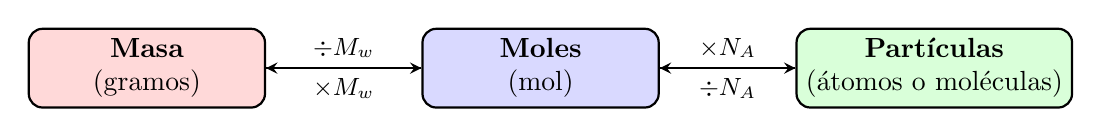
\begin{tikzpicture}[
        box/.style={rectangle, draw, thick, fill=#1, rounded corners=5pt, minimum width=3cm, minimum height=1cm, align=center},
        arr/.style={->, thick, >=stealth}
    ]
        \node[box=red!15] (masa) at (-5,0) {\textbf{Masa} \\ (gramos)};
        \node[box=blue!15] (mol) at (0,0) {\textbf{Moles} \\ (mol)};
        \node[box=green!15] (part) at (5,0) {\textbf{Partículas} \\ (átomos o moléculas)};

        \draw[arr] (masa) -- node[above, font=\small] {\( \div M_w \)} (mol);
        \draw[arr] (mol) -- node[below, font=\small] {\( \times M_w \)} (masa);
        \draw[arr] (mol) -- node[above, font=\small] {\( \times N_A \)} (part);
        \draw[arr] (part) -- node[below, font=\small] {\( \div N_A \)} (mol);
    \end{tikzpicture}
    \caption{Relación entre masa, moles, y número de partículas.}
    \label{fig:masa_mol_particulas}
\end{figure}

\begin{example}{}

    Calcula los moles de \ch{CH4} contenidos en \qty{48}{\g}.

    \datos{}: Las masas atómicas son: \( \ch{H} = 1 \); \( \ch{C} = 12 \).

    Primero debemos calcular la masa molar. Como hemos dicho, la masa molar tiene el mismo valor numérico que la masa molecular, pero en \unit{\g\per\mole} en lugar de uma.

    \[
        \ch{CH4} \left\{\rule{0pt}{0.8cm}
                     \begin{array}{lcl}
                         \ch{H} &=& 4 \times \qty{1}{\uma} = \qty{4}{\uma} \\
                         \ch{C} &=& 1 \times \qty{12}{\uma} = \qty{12}{\uma} \\
                         \cline{1-3}
                         \multicolumn{3}{r}{\textbf{Total} = \qty{16}{\uma} }
                     \end{array}
        \right.
    \]

    Por lo tanto, la masa molar del \ch{CH4} es \qty{16}{\g\per\mole}.

    Aplicando la fórmula:
    \begin{equation*}
        n = \dfrac{m}{M_w} = \dfrac{48}{16} = \qty{3}{\mole} \text{ de \ch{CH4}}
    \end{equation*}
\end{example}



\begin{exercise}
    Un matraz contiene \qty{100}{\g} de carbonato de calcio, \ch{CaCO3}. Calcula la cantidad de esta sustancia, en moles, en dicho recipiente.
    \begin{solu}
        Un matraz contiene \qty{100}{\g} de carbonato de calcio, \ch{CaCO3}. Calcula la cantidad de esta sustancia, en moles, en dicho recipiente.

        Calcula los moles en \qty{100}{\g} de \ch{CaCO3}.

        Masas atómicas: \( \ch{Ca} = 40 \); \( \ch{C} = 12 \); \( \ch{O} = 16 \).

        Masa molar del \ch{CaCO3}: \( 40 + 12 + 3 \times 16 = \qty{100}{\g\per\mole} \).

        \begin{equation*}
            n = \dfrac{m}{M_w} = \dfrac{100}{100} = \qty{1}{\mole} \text{ de \ch{CaCO3}}
        \end{equation*}
    \end{solu}
\end{exercise}

\begin{exercise}
    ¿Qué cantidad en moles de nitrógeno gaseoso, \ch{N2}, hay en \qty{56}{\g} de esta sustancia? ¿Cuántas moléculas hay? ¿Y cuántos átomos?
    \begin{solu}
        ¿Qué cantidad en moles de nitrógeno gaseoso, \ch{N2}, hay en \qty{56}{\g} de esta sustancia? ¿Cuántas moléculas hay? ¿Y cuántos átomos?

        Calcula los moles, las moléculas, y los átomos en \qty{56}{\g} de \ch{N2}.

        Masa atómica: \( \ch{N} = 14 \). Masa molar del \ch{N2}: \( 2 \times 14 = \qty{28}{\g\per\mole} \).

        \textbf{Moles:}
        \begin{equation*}
            n = \dfrac{56}{28} = \qty{2}{\mole} \text{ de \ch{N2}}
        \end{equation*}

        \textbf{Moléculas:}
        \begin{equation*}
            2\ \cancelred{\unit{\mole}} \times \num{6.022e23}\ \dfrac{\text{moléculas}}{\cancelred{\unit{\mole}}} = \num{12.044e23} = \num{1.2044e24} \text{ moléculas de \ch{N2}}
        \end{equation*}

        \textbf{Átomos:} Cada molécula de \ch{N2} tiene 2 átomos de N:
        \begin{equation*}
            \num{1.2044e24} \times 2 = \num{2.4088e24} \text{ átomos de N}
        \end{equation*}
    \end{solu}
\end{exercise}

\begin{exercise}
    Calcula las masas molares de las siguientes sustancias: bromo (\ch{Br2}), yoduro de potasio (\ch{KI}), carbonato de calcio (\ch{CaCO3}), y carbonato de sodio (\ch{Na2CO3}).
    \begin{solu}
        Calcula las masas molares de las siguientes sustancias: bromo (\ch{Br2}), yoduro de potasio (\ch{KI}), carbonato de calcio (\ch{CaCO3}), y carbonato de sodio (\ch{Na2CO3}).

        Calcula las masas molares del \ch{Br2}, \ch{KI}, \ch{CaCO3}, y \ch{Na2CO3}.

        Masas atómicas: \( \ch{Br} = 80 \); \( \ch{K} = 39 \); \( \ch{I} = 127 \); \( \ch{Ca} = 40 \); \( \ch{C} = 12 \); \( \ch{O} = 16 \); \( \ch{Na} = 23 \).
        \begin{itemize}
            \item \ch{Br2}: \( 2 \times 80 = \qty{160}{\g\per\mole} \)
            \item \ch{KI}: \( 39 + 127 = \qty{166}{\g\per\mole} \)
            \item \ch{CaCO3}: \( 40 + 12 + 3 \times 16 = \qty{100}{\g\per\mole} \)
            \item \ch{Na2CO3}: \( 2 \times 23 + 12 + 3 \times 16 = 46 + 12 + 48 = \qty{106}{\g\per\mole} \)
        \end{itemize}
    \end{solu}
\end{exercise}

\begin{exercise}
    ¿Qué cantidad de sustancia, en moles, hay en \qty{66}{\g} de dióxido de carbono, \ch{CO2}?
    \begin{solu}
        ¿Qué cantidad de sustancia, en moles, hay en \qty{66}{\g} de dióxido de carbono, \ch{CO2}?

        Calcula los moles en \qty{66}{\g} de \ch{CO2}.

        Masas atómicas: \( \ch{C} = 12 \); \( \ch{O} = 16 \).

        Masa molar del \ch{CO2}: \( 12 + 2 \times 16 = \qty{44}{\g\per\mole} \).

        \begin{equation*}
            n = \dfrac{66}{44} = \qty{1.5}{\mole} \text{ de \ch{CO2}}
        \end{equation*}
    \end{solu}
\end{exercise}

\begin{exercise}
    Calcula la masa de:
    \begin{enumerate}[label=\letraminuscula]
\item \qty{2}{\mole} de cloruro de hidrógeno, \ch{HCl}.
\item \qty{2}{\mole} de agua, \ch{H2O}.
\item \qty{1.5}{\mole} de ácido sulfúrico, \ch{H2SO4}.
\item \qty{0.5}{\mole} de cloro, \ch{Cl2}.
    \end{enumerate}
    \begin{solu}
        Calcula la masa de:
        \begin{enumerate}[label=\letraminuscula]
\item \qty{2}{\mole} de cloruro de hidrógeno, \ch{HCl}.
\item \qty{2}{\mole} de agua, \ch{H2O}.
\item \qty{1.5}{\mole} de ácido sulfúrico, \ch{H2SO4}.
\item \qty{0.5}{\mole} de cloro, \ch{Cl2}.
        \end{enumerate}

        Calcula la masa de cada sustancia. Usamos \( m = n \times M_w \).

        Masas atómicas: \( \ch{H} = 1 \); \( \ch{Cl} = 35{,}5 \); \( \ch{O} = 16 \); \( \ch{S} = 32 \).

        \begin{enumerate}[label=\letraminuscula]
\item \ch{HCl}: \( M_w = 1 + 35{,}5 = \qty{36.5}{\g\per\mole} \). \( m = 2 \times 36{,}5 = \qty{73}{\g} \).
\item \ch{H2O}: \( M_w = 2 \times 1 + 16 = \qty{18}{\g\per\mole} \). \( m = 2 \times 18 = \qty{36}{\g} \).
\item \ch{H2SO4}: \( M_w = 2 + 32 + 64 = \qty{98}{\g\per\mole} \). \( m = 1{,}5 \times 98 = \qty{147}{\g} \).
\item \ch{Cl2}: \( M_w = 2 \times 35{,}5 = \qty{71}{\g\per\mole} \). \( m = 0{,}5 \times 71 = \qty{35.5}{\g} \).
        \end{enumerate}
    \end{solu}
\end{exercise}

\begin{exercise}
    ¿Qué cantidad en moles de sustancia hay en \qty{36.5}{\g} de \ch{HCl}, en \qty{73}{\g} de \ch{HCl}, y en \qty{146}{\g} de \ch{HCl}?
    \begin{solu}
        ¿Qué cantidad en moles de sustancia hay en \qty{36.5}{\g} de \ch{HCl}, en \qty{73}{\g} de \ch{HCl}, y en \qty{146}{\g} de \ch{HCl}?

        Calcula los moles en \qty{36.5}{\g}, \qty{73}{\g}, y \qty{146}{\g} de \ch{HCl}.

        Masa molar del \ch{HCl}: \( 1 + 35{,}5 = \qty{36.5}{\g\per\mole} \).

        \begin{itemize}
            \item \( n = \dfrac{36{,}5}{36{,}5} = \qty{1}{\mole} \)
            \item \( n = \dfrac{73}{36{,}5} = \qty{2}{\mole} \)
            \item \( n = \dfrac{146}{36{,}5} = \qty{4}{\mole} \)
        \end{itemize}
    \end{solu}
\end{exercise}


\section{Ley de los gases ideales}

Las tres leyes de los gases (la Ley de Gay-Lussac, la Ley de Charles, y la Ley de Boyle-Mariotte) se pueden combinar en una sola ley llamada la \textbf{Ley de los gases ideales}. Esta ley relaciona la presión, el volumen, y la temperatura con la cantidad de sustancia en moles.

La expresión matemática de esta ley es:
\vspace{20pt}
\begin{centeredequation}
    \eqnmarkbox[blue]{presion}{p}
    \cdot
    \eqnmarkbox[red]{volumen}{V}
    =
    \eqnmarkbox[mDarkTeal]{moles}{n}
    \cdot
    \eqnmarkbox[orange]{constante}{R}
    \cdot
    \eqnmarkbox[violet]{temperatura}{T}
\end{centeredequation}
\vspace{25pt}
\annotate[yshift=1em]{left}{presion}{Presión en \unit{\atmosphere}}
\annotate[yshift=-0.5em]{below,left}{volumen}{Volumen en \unit{\litre}}
\annotate[yshift=1em]{}{moles}{número de moles}
\annotate[yshift=-2em]{below,left}{constante}{Constante de los gases ideales; R = \ctegases{}}
\annotate[yshift=-1em]{below}{temperatura}{Temperatura en \unit{\kelvin}}
\begin{exercise}
    Tenemos \qty{3}{\mole} de un gas ideal a una temperatura de \qty{300}{\kelvin} y una presión de \qty{2}{\atmosphere}. Calcula el volumen que ocupa el gas.
    \begin{solu}
        Tenemos \qty{3}{\mole} de un gas ideal a una temperatura de \qty{300}{\kelvin} y una presión de \qty{2}{\atmosphere}. Calcula el volumen que ocupa el gas.

        Calcula el volumen de \qty{3}{\mole} de gas a \qty{300}{\kelvin} y \qty{2}{\atmosphere}.

        Despejamos \( V \) de la ley de los gases ideales:
        \begin{equation*}
            V = \dfrac{nRT}{p} = \dfrac{3 \times 0{,}082 \times 300}{2} = \dfrac{73{,}8}{2} = \qty{36.9}{\litre}
        \end{equation*}
    \end{solu}
\end{exercise}
\begin{exercise}
    Un gas ideal ocupa un volumen de \qty{10}{\litre} a una presión de \qty{1.5}{\atmosphere} y una temperatura de \qty{350}{\kelvin}. ¿Cuántos moles de gas hay?
    \begin{solu}
        Un gas ideal ocupa un volumen de \qty{10}{\litre} a una presión de \qty{1.5}{\atmosphere} y una temperatura de \qty{350}{\kelvin}. ¿Cuántos moles de gas hay?

        Calcula los moles de un gas que ocupa \qty{10}{\litre} a \qty{1.5}{\atmosphere} y \qty{350}{\kelvin}.

        Despejamos \( n \):
        \begin{equation*}
            n = \dfrac{pV}{RT} = \dfrac{1{,}5 \times 10}{0{,}082 \times 350} = \dfrac{15}{28{,}7} = \qty{0.52}{\mole}
        \end{equation*}
    \end{solu}
\end{exercise}
\begin{exercise}
    ¿Qué volumen en mL ocupa un gas ideal si \qty{0.553}{\mol} están a una temperatura de \qty{1226.49}{\kelvin} y una presión de \qty{4935}{\mmHg}?
    \begin{solu}
        ¿Qué volumen en mL ocupa un gas ideal si \qty{0.553}{\mol} están a una temperatura de \qty{1226.49}{\kelvin} y una presión de \qty{4935}{\mmHg}?

        Aplicamos la ley de los gases ideales $PV = nRT$, despejando el volumen:
        \begin{equation*}
            V = \frac{nRT}{P}
        \end{equation*}
        \textbf{Paso 1: Identificar los datos.}
        \begin{align*}
            n &= \qty{0.553}{\mol} \\
            T &= \qty{1226.49}{\kelvin} \\
            P &= \qty{4935}{\mmHg} \\
            R &= \qty{0.082057}{\atm\liter\per\mol\per\kelvin}
        \end{align*}
        \textbf{Paso 2: Convertir la presión a atm.}

        La constante $R$ está expresada en unidades de atm, así que debemos convertir la presión de mmHg a atm usando el factor de conversión $\qty{1}{\atm} = \qty{760}{\mmHg}$:
        \begin{equation*}
            P = \qty{4935}{\mmHg} \times \frac{\qty{1}{\atm}}{\qty{760}{\mmHg}} = \qty{6.4934}{\atm}
        \end{equation*}
        \textbf{Paso 3: Sustituir en la ecuación y calcular $V$ en litros.}
        \begin{equation*}
            V = \frac{nRT}{P} = \frac{\qty{0.553}{\mol} \times \qty{0.082057}{\atm\liter\per\mol\per\kelvin} \times \qty{1226.49}{\kelvin}}{\qty{6.4934}{\atm}} = \qty{8.573}{\liter}
        \end{equation*}
        \textbf{Paso 4: Convertir el volumen a mL.}

        Como el problema pide el volumen en mL, usamos el factor de conversión $\qty{1}{\liter} = \qty{1000}{\mL}$:
        \begin{equation*}
            V = \qty{8.573}{\liter} \times \frac{\qty{1000}{\mL}}{\qty{1}{\liter}} = \boxed{\qty{8573}{\mL}}
        \end{equation*}
    \end{solu}
\end{exercise}
\begin{exercise}
    ¿Cuál es la temperatura en \unit{\kelvin} de un gas ideal, si \qty{0.405}{\mole} ocupan un volumen de \qty{7720}{\mL} a una presión de \qty{790}{\mmHg}?
    \begin{solu}
        ¿Cuál es la temperatura en \unit{\kelvin} de un gas ideal, si \qty{0.405}{\mole} ocupan un volumen de \qty{7720}{\mL} a una presión de \qty{790}{\mmHg}?

        Aplicamos la ley de los gases ideales $PV = nRT$, despejando la temperatura:
        \begin{equation*}
            T = \frac{PV}{nR}
        \end{equation*}
        \textbf{Paso 1: Identificar los datos.}
        \begin{align*}
            n &= \qty{0.405}{\mol} \\
            V &= \qty{7720}{\mL} \\
            P &= \qty{790}{\mmHg} \\
            R &= \qty{0.082057}{\atm\liter\per\mol\per\kelvin}
        \end{align*}
        \textbf{Paso 2: Convertir la presión a atm.}

        Convertimos mmHg a atm usando el factor de conversión $\qty{1}{\atm} = \qty{760}{\mmHg}$:
        \begin{equation*}
            P = \qty{790}{\mmHg} \times \frac{\qty{1}{\atm}}{\qty{760}{\mmHg}} = \qty{1.03947}{\atm}
        \end{equation*}
        \textbf{Paso 3: Convertir el volumen a litros.}

        La constante $R$ tiene litros en sus unidades, así que convertimos mL a L usando el factor de conversión $\qty{1}{\liter} = \qty{1000}{\mL}$:
        \begin{equation*}
            V = \qty{7720}{\mL} \times \frac{\qty{1}{\liter}}{\qty{1000}{\mL}} = \qty{7.720}{\liter}
        \end{equation*}
        \textbf{Paso 4: Sustituir en la ecuación y calcular $T$.}
        \begin{equation*}
            T = \frac{PV}{nR} = \frac{\qty{1.03947}{\atm} \times \qty{7.720}{\liter}}{\qty{0.405}{\mol} \times \qty{0.082057}{\atm\liter\per\mol\per\kelvin}} = \boxed{\qty{241.5}{\kelvin}}
        \end{equation*}
    \end{solu}
\end{exercise}
\begin{exercise}
    ¿Cuál es la temperatura en \unit{\degreeCelsius} de un gas ideal, si \qty{0.746}{\mol} ocupan un volumen de \qty{9890}{\mL} a una presión de \qty{1.41}{\atmosphere}?
    \begin{solu}
        ¿Cuál es la temperatura en \unit{\degreeCelsius} de un gas ideal, si \qty{0.746}{\mol} ocupan un volumen de \qty{9890}{\mL} a una presión de \qty{1.41}{\atmosphere}?

        Aplicamos la ley de los gases ideales $PV = nRT$, despejando la temperatura:
        \begin{equation*}
            T = \frac{PV}{nR}
        \end{equation*}
        \textbf{Paso 1: Identificar los datos.}
        \begin{align*}
            n &= \qty{0.746}{\mol} \\
            V &= \qty{9890}{\mL} \\
            P &= \qty{1.41}{\atm} \\
            R &= \qty{0.082057}{\atm\liter\per\mol\per\kelvin}
        \end{align*}
        \textbf{Paso 2: Convertir el volumen a litros.}

        Convertimos mL a L usando el factor de conversión $\qty{1}{\liter} = \qty{1000}{\mL}$:
        \begin{equation*}
            V = \qty{9890}{\mL} \times \frac{\qty{1}{\liter}}{\qty{1000}{\mL}} = \qty{9.890}{\liter}
        \end{equation*}
        \textbf{Paso 3: Sustituir en la ecuación y calcular $T$ en Kelvin.}
        \begin{equation*}
            T = \frac{PV}{nR} = \frac{\qty{1.41}{\atm} \times \qty{9.890}{\liter}}{\qty{0.746}{\mol} \times \qty{0.082057}{\atm\liter\per\mol\per\kelvin}} = \qty{227.8}{\kelvin}
        \end{equation*}
        \textbf{Paso 4: Convertir la temperatura a \unit{\degreeCelsius}.}

        El problema pide la temperatura en \unit{\degreeCelsius}. Usamos la relación $T(\unit{\degreeCelsius}) = T(\unit{\kelvin}) - 273.15$:
        \begin{equation*}
            T = \qty{227.8}{\kelvin} - \qty{273.15}{\kelvin} = \boxed{\qty{-45.35}{\degreeCelsius}}
        \end{equation*}
    \end{solu}
\end{exercise}
\begin{exercise}
    ¿Cuál es la presión en atm de un gas ideal si \qty{0.532}{\mol} ocupan un volumen de \qty{4390}{\mL} a una temperatura de \qty{183.93}{\kelvin}?
    \begin{solu}
        ¿Cuál es la presión en atm de un gas ideal si \qty{0.532}{\mol} ocupan un volumen de \qty{4390}{\mL} a una temperatura de \qty{183.93}{\kelvin}?

        Aplicamos la ley de los gases ideales $PV = nRT$, despejando la presión:
        \begin{equation*}
            P = \frac{nRT}{V}
        \end{equation*}
        \textbf{Paso 1: Identificar los datos.}
        \begin{align*}
            n &= \qty{0.532}{\mol} \\
            V &= \qty{4390}{\mL} \\
            T &= \qty{183.93}{\kelvin} \\
            R &= \qty{0.082057}{\atm\liter\per\mol\per\kelvin}
        \end{align*}
        \textbf{Paso 2: Convertir el volumen a litros.}

        Convertimos mL a L usando el factor de conversión $\qty{1}{\liter} = \qty{1000}{\mL}$:
        \begin{equation*}
            V = \qty{4390}{\mL} \times \frac{\qty{1}{\liter}}{\qty{1000}{\mL}} = \qty{4.390}{\liter}
        \end{equation*}
        \textbf{Paso 3: Sustituir en la ecuación y calcular $P$.}
        \begin{equation*}
            P = \frac{nRT}{V} = \frac{\qty{0.532}{\mol} \times \qty{0.082057}{\atm\liter\per\mol\per\kelvin} \times \qty{183.93}{\kelvin}}{\qty{4.390}{\liter}} = \boxed{\qty{1.829}{\atm}}
        \end{equation*}
    \end{solu}
\end{exercise}
\begin{exercise}
    ¿Cuántos moles de un gas ideal hay en un volumen de \qty{4220}{\mL} si la temperatura es \qty{279.35}{\kelvin} y la presión es \qty{1.75}{\atmosphere}?
    \begin{solu}
        ¿Cuántos moles de un gas ideal hay en un volumen de \qty{4220}{\mL} si la temperatura es \qty{279.35}{\kelvin} y la presión es \qty{1.75}{\atmosphere}?

        Aplicamos la ley de los gases ideales $PV = nRT$, despejando el número de moles:
        \begin{equation*}
            n = \frac{PV}{RT}
        \end{equation*}
        \textbf{Paso 1: Identificar los datos.}
        \begin{align*}
            V &= \qty{4220}{\mL} \\
            T &= \qty{279.35}{\kelvin} \\
            P &= \qty{1.75}{\atm} \\
            R &= \qty{0.082057}{\atm\liter\per\mol\per\kelvin}
        \end{align*}
        \textbf{Paso 2: Convertir el volumen a litros.}

        Convertimos mL a L usando el factor de conversión $\qty{1}{\liter} = \qty{1000}{\mL}$:
        \begin{equation*}
            V = \qty{4220}{\mL} \times \frac{\qty{1}{\liter}}{\qty{1000}{\mL}} = \qty{4.220}{\liter}
        \end{equation*}
        \textbf{Paso 3: Sustituir en la ecuación y calcular $n$.}
        \begin{equation*}
            n = \frac{PV}{RT} = \frac{\qty{1.75}{\atm} \times \qty{4.220}{\liter}}{\qty{0.082057}{\atm\liter\per\mol\per\kelvin} \times \qty{279.35}{\kelvin}} = \boxed{\qty{0.3223}{\mol}}
        \end{equation*}
    \end{solu}
\end{exercise}

\subsection{Condiciones normales (CN)}

En química, es muy habitual hablar de condiciones normales.
Cuando hablamos de condiciones normales, nos referimos a una presión de \qty{1}{\atmosphere} y una temperatura de \qty{0}{\degreeCelsius} (\qty{273}{\kelvin}).

Es importante saber que \qty{1}{\mol} de \textbf{cualquier gas} en condiciones normales siempre ocupa un volumen de \qty{22.4}{\litre}. Este volumen se llama \textbf{volumen molar}.

Para comprobar este valor, solo necesitamos aplicar la ecuación de los gases ideales con \( n=1 \), \( p = \qty{1}{\atmosphere} \), y \( T = \qty{273}{\kelvin} \):
\begin{centeredequation}
    V = \dfrac{nRT}{p} = \dfrac{1 \times 0{,}082 \times 273}{1} = \qty{22.4}{\litre}
\end{centeredequation}
\begin{exercise}
    ¿Qué volumen ocupan \qty{2}{\mole} de oxígeno (\ch{O2}) en condiciones normales?
    \begin{solu}
        ¿Qué volumen ocupan \qty{2}{\mole} de oxígeno (\ch{O2}) en condiciones normales?

        Volumen de \qty{2}{\mole} de \ch{O2} en CN.

        En condiciones normales, 1 mol de cualquier gas ocupa \qty{22.4}{\litre}:
        \begin{equation*}
            V = 2\ \cancelred{\unit{\mole}} \times \dfrac{\qty{22.4}{\litre}}{1\ \cancelred{\unit{\mole}}} = \qty{44.8}{\litre}
        \end{equation*}
    \end{solu}
\end{exercise}
\begin{exercise}
    ¿Cuántos moles de un gas ideal hay en \qty{11.2}{\litre} en condiciones normales?
    \begin{solu}
        ¿Cuántos moles de un gas ideal hay en \qty{11.2}{\litre} en condiciones normales?

        Moles en \qty{11.2}{\litre} de gas en CN.

        \begin{equation*}
            n = \dfrac{11{,}2}{22{,}4} = \qty{0.5}{\mole}
        \end{equation*}
    \end{solu}
\end{exercise}
\begin{exercise}
    ¿Qué volumen en mL ocupan \qty{0.553}{\mol} de un gas ideal en CN?
    \begin{solu}
        ¿Qué volumen en mL ocupan \qty{0.553}{\mol} de un gas ideal en CN?

        Las condiciones normales (CN) corresponden a una temperatura de $T = \qty{273.15}{\kelvin}$
        y una presión de $P = \qty{1}{\atm}$. En estas condiciones, podemos calcular el
        volumen molar de un gas ideal a partir de la ley de los gases ideales $PV = nRT$:
        \begin{equation*}
            V_m = \frac{RT}{P} = \frac{\qty{0.082057}{\atm\liter\per\mol\per\kelvin}
            \times \qty{273.15}{\kelvin}}{\qty{1}{\atm}} = \qty{22.414}{\liter\per\mol}
        \end{equation*}
        Este valor se conoce como el \textbf{volumen molar en condiciones normales} y nos permite
        calcular directamente el volumen de cualquier cantidad de gas ideal en CN usando la
        relación:
        \begin{equation*}
            V = n \times V_m
        \end{equation*}
        \textbf{Paso 1: Identificar los datos.}
        \begin{align*}
            n   &= \qty{0.553}{\mol} \\
            V_m &= \qty{22.414}{\liter\per\mol}
        \end{align*}
        \textbf{Paso 2: Calcular el volumen en litros.}
        \begin{equation*}
            V = n \times V_m = \qty{0.553}{\mol} \times \qty{22.414}{\liter\per\mol}
            = \qty{12.395}{\liter}
        \end{equation*}
        \textbf{Paso 3: Convertir el volumen a mL.}

        El problema pide el volumen en mL, así que usamos el factor de conversión
        $\qty{1}{\liter} = \qty{1000}{\mL}$:
        \begin{equation*}
            V = \qty{12.395}{\liter} \times \frac{\qty{1000}{\mL}}{\qty{1}{\liter}}
            = \boxed{\qty{12395}{\mL}}
        \end{equation*}
    \end{solu}
\end{exercise}
\begin{exercise}
    ¿Cuántos moles de un gas ideal hay en un volumen de \qty{7720}{\mL} en CN?
    \begin{solu}
        ¿Cuántos moles de un gas ideal hay en un volumen de \qty{7720}{\mL} en CN?

        En condiciones normales (CN), $T = \qty{273.15}{\kelvin}$ y $P = \qty{1}{\atm}$,
        el volumen molar de un gas ideal es $V_m = \qty{22.414}{\liter\per\mol}$. Despejando
        el número de moles de la relación $V = n \times V_m$:
        \begin{equation*}
            n = \frac{V}{V_m}
        \end{equation*}
        \textbf{Paso 1: Identificar los datos.}
        \begin{align*}
            V   &= \qty{7720}{\mL} \\
            V_m &= \qty{22.414}{\liter\per\mol}
        \end{align*}
        \textbf{Paso 2: Convertir el volumen a litros.}

        La constante $V_m$ está expresada en \unit{\liter\per\mol}, así que debemos convertir
        el volumen de mL a L usando el factor de conversión
        $\qty{1}{\liter} = \qty{1000}{\mL}$:
        \begin{equation*}
            V = \qty{7720}{\mL} \times \frac{\qty{1}{\liter}}{\qty{1000}{\mL}}
            = \qty{7.720}{\liter}
        \end{equation*}
        \textbf{Paso 3: Calcular el número de moles.}
        \begin{equation*}
            n = \frac{V}{V_m} = \frac{\qty{7.720}{\liter}}{\qty{22.414}{\liter\per\mol}}
            = \boxed{\qty{0.3444}{\mol}}
        \end{equation*}
    \end{solu}
\end{exercise}
\begin{exercise}
    ¿Qué volumen en \unit{\liter} ocupan \qty{0.746}{\mol} de un gas ideal en CN?
    \begin{solu}
        ¿Qué volumen en \unit{\liter} ocupan \qty{0.746}{\mol} de un gas ideal en CN.

        \negsubro{SOLUCIÓN:}

        En condiciones normales (CN), $T = \qty{273.15}{\kelvin}$ y $P = \qty{1}{\atm}$,
        el volumen molar de un gas ideal es $V_m = \qty{22.414}{\liter\per\mol}$. El volumen
        ocupado por una cantidad $n$ de gas ideal se calcula mediante:
        \begin{equation*}
            V = n \times V_m
        \end{equation*}
        \textbf{Paso 1: Identificar los datos.}
        \begin{align*}
            n   &= \qty{0.746}{\mol} \\
            V_m &= \qty{22.414}{\liter\per\mol}
        \end{align*}
        \textbf{Paso 2: Calcular el volumen en litros.}

        Como el problema pide el resultado directamente en litros, no es necesaria ninguna
        conversión de unidades:
        \begin{equation*}
            V = n \times V_m = \qty{0.746}{\mol} \times \qty{22.414}{\liter\per\mol}
            = \boxed{\qty{16.721}{\liter}}
        \end{equation*}
    \end{solu}
\end{exercise}
\begin{exercise}
    ¿Cuántos moles de un gas ideal hay en un volumen de \qty{4390}{\mL} en CN?
    \begin{solu}
        ¿Cuántos moles de un gas ideal hay en un volumen de \qty{4390}{\mL} en CN?

        \negsubro{SOLUCIÓN:}

        En condiciones normales (CN), $T = \qty{273.15}{\kelvin}$ y $P = \qty{1}{\atm}$,
        el volumen molar de un gas ideal es $V_m = \qty{22.414}{\liter\per\mol}$. Despejando
        el número de moles de la relación $V = n \times V_m$:
        \begin{equation*}
            n = \frac{V}{V_m}
        \end{equation*}
        \textbf{Paso 1: Identificar los datos.}
        \begin{align*}
            V   &= \qty{4390}{\mL} \\
            V_m &= \qty{22.414}{\liter\per\mol}
        \end{align*}
        \textbf{Paso 2: Convertir el volumen a litros.}

        Convertimos mL a L usando el factor de conversión $\qty{1}{\liter} = \qty{1000}{\mL}$:
        \begin{equation*}
            V = \qty{4390}{\mL} \times \frac{\qty{1}{\liter}}{\qty{1000}{\mL}}
            = \qty{4.390}{\liter}
        \end{equation*}
        \textbf{Paso 3: Calcular el número de moles.}
        \begin{equation*}
            n = \frac{V}{V_m} = \frac{\qty{4.390}{\liter}}{\qty{22.414}{\liter\per\mol}}
            = \boxed{\qty{0.1959}{\mol}}
        \end{equation*}
    \end{solu}
\end{exercise}
\begin{exercise}
    ¿Qué volumen en mL ocupan \qty{1.75}{\mol} de un gas ideal en CN?
    \begin{solu}
        ¿Qué volumen en mL ocupan \qty{1.75}{\mol} de un gas ideal en CN?

        \negsubro{SOLUCIÓN:}

        En condiciones normales (CN), $T = \qty{273.15}{\kelvin}$ y $P = \qty{1}{\atm}$,
        el volumen molar de un gas ideal es $V_m = \qty{22.414}{\liter\per\mol}$. El volumen
        ocupado por una cantidad $n$ de gas ideal se calcula mediante:
        \begin{equation*}
            V = n \times V_m
        \end{equation*}
        \textbf{Paso 1: Identificar los datos.}
        \begin{align*}
            n   &= \qty{1.75}{\mol} \\
            V_m &= \qty{22.414}{\liter\per\mol}
        \end{align*}
        \textbf{Paso 2: Calcular el volumen en litros.}
        \begin{equation*}
            V = n \times V_m = \qty{1.75}{\mol} \times \qty{22.414}{\liter\per\mol}
            = \qty{39.225}{\liter}
        \end{equation*}
        \textbf{Paso 3: Convertir el volumen a mL.}

        El problema pide el volumen en mL, así que usamos el factor de conversión
        $\qty{1}{\liter} = \qty{1000}{\mL}$:
        \begin{equation*}
            V = \qty{39.225}{\liter} \times \frac{\qty{1000}{\mL}}{\qty{1}{\liter}}
            = \boxed{\qty{39225}{\mL}}
        \end{equation*}
    \end{solu}
\end{exercise}


%\section{Vocabulario}
%
%\begin{vocabulary}[Valence electrons]
%    Electrons in the outermost shell of an atom which are responsible for the chemical properties of an element. \newline
%    \textbf{Translation to Spanish}: Electrones de valencia \newline
%    % 248
%\end{vocabulary}
%
%\begin{vocabulary}[Chemical compound]
%    Substance formed by two or more different elements that are chemically bonded together in fixed and specific proportions. \newline
%    \textbf{Translation to Spanish}: Compuesto químico \newline
%    % 271
%\end{vocabulary}
%
%\begin{vocabulary}[Molecule]
%    The smallest possible unit of a chemical substance that still retains all of its unique and characteristic properties. \newline
%    \textbf{Translation to Spanish}: Molécula \newline
%    % 273
%\end{vocabulary}
%
%\begin{vocabulary}[Isolated atoms]
%    Atoms found in noble gases that do not tend to combine with others because their valence shell is complete. \newline
%    \textbf{Translation to Spanish}: Átomos aislados \newline
%    % 275
%\end{vocabulary}
%
%\begin{vocabulary}[Noble gases]
%    Highly stable elements that do not conduct electricity or react with other substances due to their complete shells. \newline
%    \textbf{Translation to Spanish}: Gases nobles \newline
%    % 276
%\end{vocabulary}
%
%\begin{vocabulary}[Homonuclear diatomic molecules]
%    Molecules formed by the union of two atoms of the same chemical element, such as oxygen or hydrogen. \newline
%    \textbf{Translation to Spanish}: Moléculas diatómicas homonucleares \newline
%    % 280
%\end{vocabulary}
%
%\begin{vocabulary}[Heteronuclear molecules]
%    Specific types of molecules that contain two or more different elements chemically bonded together in a single unit. \newline
%    \textbf{Translation to Spanish}: Moléculas heteronucleares \newline
%    % 282
%\end{vocabulary}
%
%\begin{vocabulary}[Crystals]
%    Solids whose internal particles are arranged following a pattern that repeats in all three dimensions of physical space. \newline
%    \textbf{Translation to Spanish}: Cristales \newline
%    % 283
%\end{vocabulary}
%
%\begin{vocabulary}[Chemical bond]
%    The union between atoms of different elements that occurs because the molecule formed is more stable than others. \newline
%    \textbf{Translation to Spanish}: Enlace químico \newline
%    % 317
%\end{vocabulary}
%
%\begin{vocabulary}[Ionic bond]
%    Bond that occurs by electron transfer where one element loses electrons and another gains them, forming stable ions. \newline
%    \textbf{Translation to Spanish}: Enlace iónico \newline
%    % 318
%\end{vocabulary}
%
%\begin{vocabulary}[Cation]
%    A positive ion formed when a neutral atom loses one or more electrons during a chemical reaction process. \newline
%    \textbf{Translation to Spanish}: Catión \newline
%    % 319
%\end{vocabulary}
%
%\begin{vocabulary}[Anion]
%    A negative ion formed when a neutral atom gains one or more electrons during a chemical reaction process. \newline
%    \textbf{Translation to Spanish}: Anión \newline
%    % 319
%\end{vocabulary}
%
%\begin{vocabulary}[Covalent bond]
%    The specific type of chemical bond that forms when two atoms share electrons to complete their outermost shell. \newline
%    \textbf{Translation to Spanish}: Enlace covalente \newline
%    % 343
%\end{vocabulary}
%
%\begin{vocabulary}[Metallic bond]
%    Bond between atoms of metallic elements where valence electrons move freely, forming a large and common electron cloud. \newline
%    \textbf{Translation to Spanish}: Enlace metálico \newline
%    % 364
%\end{vocabulary}
%
%\begin{vocabulary}[Electron cloud]
%    The zone in metallic bonds where valence electrons move freely among all the atoms, allowing electrical conduction. \newline
%    \textbf{Translation to Spanish}: Nube electrónica \newline
%    % 364
%\end{vocabulary}
%
%\begin{vocabulary}[Graphite]
%    A non-metallic crystal formed by carbon atoms arranged in stacked hexagonal layers that are soft and opaque. \newline
%    \textbf{Translation to Spanish}: Grafito \newline
%    % 296
%\end{vocabulary}
%
%
